\chapter{Standardization}

\section{Problem Statement}
The standardization process is a process to convert the instrumental values to physical values. In CCD, what is being read is the potential ($ \propto $ number of electrons $ \propto $ flux). But what does a CCD pixel value mean? $ 1 $ ADU can mean $ \SI{1}{Jy} $ at one CCD but at different one it can mean $ \SI{5}{Jy} $ because it is designed to be insensitive to photons for some reason. Thus, what astronomers do is

\begin{enumerate}
\item Make a list of objects which have known flux (e.g., star A has spectrum of blahblah, and it has $ \mathrm{V}_\mathrm{std} $ magnitude or flux $ I_\mathrm{std} $ in the V-band). These stars are called \textbf{standard stars}.
\item Observe the target and the standard stars simultaneously. If they cannot be in the same field of view, observe them at the same night when airmasses are not too different and weather is not changed largely.
\end{enumerate}
Now the power of CCD comes in: It's highly linear, i.e., the pixel counts of $ N $ (of the target of interest) and $ N_\mathrm{std} $ are very much proportional to the original flux, $ I $ and $ I_0 $. Thus, you can use Pogson's formula, because what it requires is only the ratio of flux: 
\begin{equation}\label{eq: Pogson}
  \mathrm{V} - \mathrm{V}_\mathrm{std} 
    = -2.5 \lg \frac{I}{I_\mathrm{std}} 
    =  -2.5 \lg \frac{N}{N_\mathrm{std}} ~.
\end{equation}

\begin{ex}[Simplest Standardization]
If the aperture photometry gave pixel count of $ 1000 $ for a standard star of $ \mathrm{V}_\mathrm{std} = \m{10.00} $ and the object had pixel count of $ 500 $, the above formula will give $ \mathrm{V} = \m{10.75} $. 
\end{ex}

In practice\footnote{From here, I extensively refered to Ch. 6 of ``A Practical Guide to Lightcurve Photometry and Analysis'' by Brian D. Warner, 2e.}, especially when stars with catalogued magnitude are not in the same field of view as the target of interest, it is very difficult to use these formulae. In such a case, we have two FITS images to compare: one for target and one for standard star (usually far away from the target). A direct comparison of $ N $ and $ N_0 $ is difficult because
\begin{enumerate}
\item The atmosphre exists. The magnitude we observe on ground is different from the one we would have observed outside of the atmosphere (space). This gives the $ k' $ and $ k'' $ terms in \cref{eq: std} below.
\item The CCD is not ideally simple. For example, if it is more sensitive to redder wavelength, making red stars brighter than they should be. This gives the $ k $ term in \cref{eq: std} below.
\end{enumerate}
If all these are considered with proper approximations (derived later in this chapter), we can obtain the following second-order approximation of the standard magnitude of an object seen on CCD:
\begin{equation}\label{eq: std}
\begin{aligned}
  M_f &= m_f + (\mathrm{effect\ of\ atmosphere}) + (\mathrm{effect\ of\ CCD}) \\
    &\approx m_f - k_f' X - k_f''XC + z_f + k_f C \\
    &\equiv m_{0f} + z_f + k_f C ~,
\end{aligned}
\end{equation}
where
\begin{equation}
  m_{f} \equiv m_{0f} + k_f'X + k_f'' XC
\end{equation}
and
\begin{itemize}
\item $ f $: The filter (V, B, g', etc).
\item $ X $: airmass (the simplest approximation is the secant of zenith angle, $ \sec Z $).
\item $ M_f $: The \emph{standard} apparent magnitude (or the \emph{true} apparent magnitude) at filter $ f $.
\item $ m_f $: The \emph{instrumental} magnitude ($ m_f = -2.5 \lg N $).
\item $ m_{0f} $: The extra-atmospheric magnitude ($ m_f $ value we would have obtained if we were in space $ X = 0 $).
\item $ C $: The \emph{true} color index\footnote{Not necessarily include filter $ f $, but it is better that the wavelength ranges of the selected two filters ``contain'' the range of $ f $ for interpolation purpose.}, e.g., $ \mathrm{B} - \mathrm{V} $ or $ \mathrm{r'} - \mathrm{i'} $.
\item $ k_f' $: The first order extinction coefficient at filter $ f $.
\item $ k_f'' $: The second order extinction coefficient at filter $ f $.
\item $ z_f $: The zero point at filter $ f $.
\item $ k_f $: The system transform coefficient at filter $ f $.
\item Note: lower- and upper-cased letters are used for the \emph{instrumental} and \emph{true} magnitudes, respectively\footnote{For example, v, b, $ m_\mathrm{g'} $ are instrumental magnitudes of an object and V, B, and $ M_\mathrm{g'} $ are true appparent magnitudes of it.}.
\end{itemize}

%The example I showed with \cref{eq: Pogson} is the case when $ k_f = k_f' = k_f'' = 0 $, or equivalently $ k_f = 0 $ and $ X = 0 $. In such a case, the true apparent magnitude is $ \mathrm{V} = \mathrm{v} + z_\mathrm{V} = -2.5 \lg N + z_\mathrm{V} $ where $ \mathrm{v} $ is the instrumental magnitude and $ z_\mathrm{V} $ is just a constant\footnote{}. Same goes true for the standard star, so $ \mathrm{V}_0 = \mathrm{v}_0 + z_\mathrm{V} = -2.5 \lg N_0 + Z_\mathrm{V} $. Then \cref{eq: Pogson} makes sense and $ \mathrm{V}- \mathrm{V}_0 = \mathrm{v} - \mathrm{v}_0 $. If the coefficients are non-zero, you can see that 

From \cref{eq: std}:
\begin{equation}
  \mathrm{V} - \mathrm{V}_\mathrm{std}
    = (\mathrm{v} - \mathrm{v}_\mathrm{std})
    + k_\mathrm{V}'(X - X_\mathrm{std})
    + k_\mathrm{V}''(X C - X_\mathrm{std} C_\mathrm{std})
    + k_\mathrm{V}(C - C_\mathrm{std})
    + \Delta z_\mathrm{V}
    \neq \mathrm{v} - \mathrm{v}_\mathrm{std} ~.
\end{equation}
So the calculation given in the example is true only if the airmass of the object and standard star are identical AND the true color indices of them are identical. Otherwise, we cannot simply equate the right hand side of \cref{eq: Pogson} ($ = \mathrm{v} - \mathrm{v}_\mathrm{std} $) to the left hand side ($ = \mathrm{V} - \mathrm{V}_\mathrm{std} $). In space, we can remove all the atmosphere related terms since $ X = 0 $. Also $ \Delta z \approx 0 $ is assumed (discussed in \cref{ss: zeropt}), so only the $ k_f $ term remains. This is why space observation is powerful.

\section{Understanding the Standardization Formula}
In this section, I will discuss about the terms in \cref{eq: std} with some realistic data and plots. At the same time, I will give a derivation of the equation. Many textbooks only give the former; I do not want to go against that trend, but I wanted more quantitative explanations and justifications of those at the same time. 

\subsection{Atmospheric Extinction}
The atmospheric extinction is dependent on the wavelength as in \cref{fig:air-ext-and-filter}. The extinction is expressed as mag/airmass, i.e., the extincted magnitude when airmass $ X = 1 $, i.e., ``$ m_f - m_{0f} $ at $ X = 1 $'' or $ k_f' + k_f''C $ in the language of \cref{eq: std}. The extinction is severe at shorter wavelengths, and that is why the Sun looks redder when it rises or sets (i.e., when airmass is larger). 

\begin{figure}[ht!]
\centering
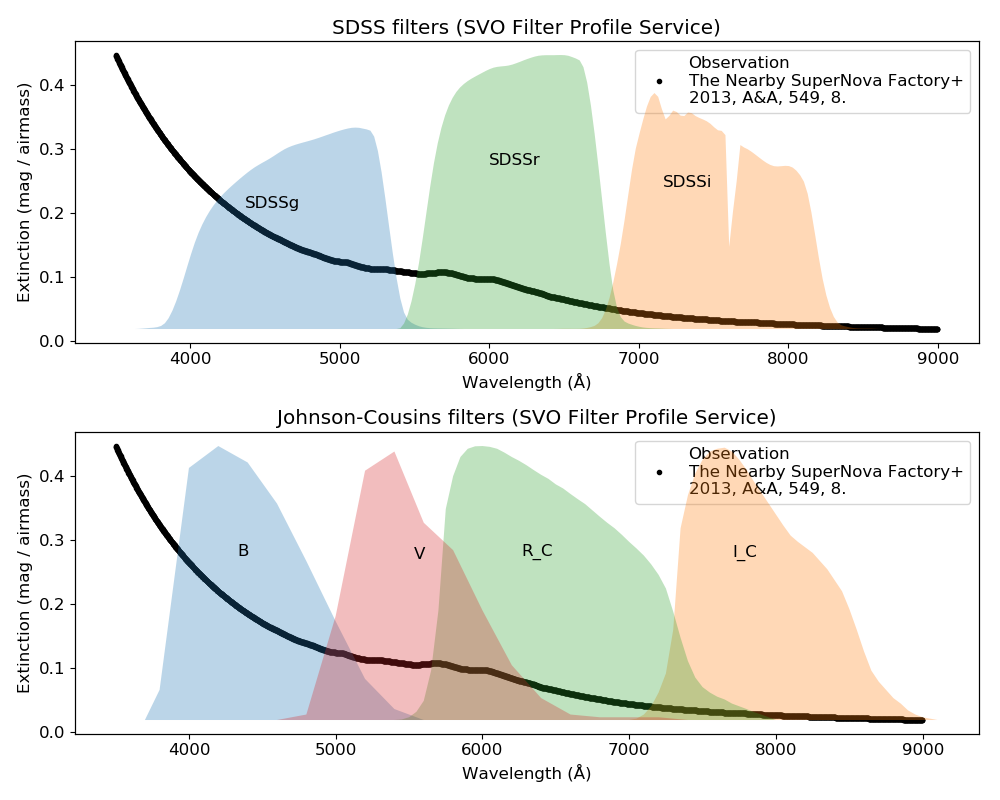
\includegraphics[width=0.9\linewidth]{figs/air-ext-and-filter}
\caption{The atmospheric extinction as a function of wavelength at Mauna Kea, \textit{based on some 4285 standard star spectra obtained on 478 nights spread over a period of 7 years obtained by the Nearby SuperNova Factory using the SuperNova Integral Field Spectrograph.} (excerpt from The Nearby SuperNova Factory+ 2013, A\&A, 549, 8). The SDSS and Johnson-Cousins filters' filter profiles are overplotted.}
\label{fig:air-ext-and-filter}
\end{figure}

Consider an object with spectrum $ S_0(\lambda) $, measured at space, is observed at an airmass of $ X $. The intensity at filter with profile $ f_f(\lambda) $ without atmosphere is $ \int_{0}^{\infty} S_0(\lambda) f_f(\lambda) d\lambda $. Because $ f_f(\lambda) $ can be set as non-zero for $ \lambda \in (\lambda_1, \lambda_2) $ and 0 otherwise, it can also be written as $ \int_{\lambda_1}^{\lambda_2} S_0(\lambda) f_f(\lambda) d\lambda $. If the spectrum undergoes atmospheric extinction described by optical depth of $ \tau(\lambda) $, the intensity after the filter throughput is $ \int_{\lambda_1}^{\lambda_2} S_0(\lambda) f_f(\lambda)  e^{-\int \tau(\lambda) dX} d\lambda \approx \int_{\lambda_1}^{\lambda_2} S_0(\lambda) f_f(\lambda)  e^{-\tau(\lambda) X} d\lambda$, where $ e^{-\tau(\lambda) X} $ is an approximation of $ e^{\int -\tau(\lambda) dX} $, where the integration is along the optical path along the atmosphere. When extinction is not severe, i.e., $ \tau(\lambda) X \ll 1 $ for all $ \lambda $ of interest, $ e^{-\tau(\lambda) X} \approx 1 - \tau(\lambda) X $ (approx 1). Also when $ A \ll 1 $, $ \lg (1 - A) \approx - A / \ln 10 $ (approx 2). Combining these information, Pogson's formula states
\begin{equation}
\begin{aligned}
  m_f - m_{0f}
    &= -2.5 \lg
      \qty( \frac{\int_{\lambda_1}^{\lambda_2} S_0(\lambda) f(\lambda) e^{-\tau(\lambda) X} d\lambda}
      {\int_{\lambda_1}^{\lambda_2} S_0(\lambda) f(\lambda) d\lambda} ) \\
    \mathrm{(using\ approx\ 1)}
    &\approx -2.5 \lg 
      \qty( 1 - \frac{\int_{\lambda_1}^{\lambda_2} S_0(\lambda) f(\lambda) \tau(\lambda) d\lambda}
        {\int_{\lambda_1}^{\lambda_2} S_0(\lambda) f(\lambda) d\lambda} X ) \\
    \mathrm{(using\ approx\ 2)}
    &\approx \frac{2.5}{\ln 10} 
      \frac{\int_{\lambda_1}^{\lambda_2} S_0(\lambda) f(\lambda) \tau(\lambda) d\lambda}
        {\int_{\lambda_1}^{\lambda_2} S_0(\lambda) f(\lambda) d\lambda} X ~.
\end{aligned}
\end{equation}

Remembering $ I(\lambda) = I_0(\lambda) e^{-\tau(\lambda) X} $, we have extinction (magnitude)
\begin{equation*}
  \Delta m(\lambda) 
    = -2.5 \lg \qty( \frac{I(\lambda)}{I_0(\lambda)} ) 
    = 1.086 \tau(\lambda) X ~.
\end{equation*} 
Then the $ y $-axis of \cref{fig:air-ext-and-filter} is $ 1.086 \tau(\lambda) $, so you can roughly understand that the $ y $-axis represents $ \tau(\lambda) $. Hence, $ \tau(\lambda) X \ll 1 $ (approx 1) is reasonable. In cases such as short wavelength (shorter than B/g) and high airmass observation, this assumption may break down. This is why classical photometric observers dislike observations at airmass $ X \gtrsim 1.5\mathrm{-}2 $ which corresponds to elevation smaller than $ 48^\circ \mathrm{-} 30^\circ$. For polarimetry, however, only the \emph{ratio} of two electric field vector directions are important, so airmass does not matter\footnote{For example, \texttt{ItoT+2018, NatCo, 9, 2486} demonstrated the polarization degree is not seriously affected by airmass even up to 7 compared to that of 1.03, at least less than 0.05 \%p. This is because atmospheric scattering is basically a \emph{forward} scattering, which should not induce any additional polarization degree although the total intensity should decrease.} The error due to the approximation, however, may not be severe compared to other error sources (e.g., changing weather). 

Now we want to further assume that, $ \tau(\lambda) \approx \tilde{c}_1 + \tilde{c}_2 \lambda $ within the wavelength range of $ (\lambda_1, \lambda_2) $. This is similar to approximating the black markers in \cref{fig:air-ext-and-filter} within each filter as a line because its y-axis is nothing but $ 1.086 \tau $. Then
\begin{equation}
  m_f - m_{0f} 
    \approx 2.5 
    \qty (c_1 + c_2\frac{\int_{\lambda_1}^{\lambda_2} S_0(\lambda) f(\lambda) \lambda d\lambda}
      {\int_{\lambda_1}^{\lambda_2} S_0(\lambda) f(\lambda) d\lambda} ) X ~.
\end{equation}
Here, $ c_1 $ and $ c_2 $ are also constants. If the filter is fixed (e.g., V-band or SDSS $ \mathrm{g'} $ filter, etc), the only unknown thing in the second term in the parentheses is $ S_0(\lambda) $, i.e., the spectral shape. If it is a black body spectrum, the shape of $ S_0 $ is determined uniquely once the color index $ C $ is known. Even if it is not a perfect black body, it is reasonable to assume the spectral shape, $ S_0(\lambda) $, and color index, $ C $, have \textit{nearly} one-to-one relationship\footnote{For example, if you look at the color-color diagram of stars, A0, F0, and G0 stars all share similar $ \mathrm{U} - \mathrm{B} $ colors, i.e., color index and spectral shape are not one-to-one. This happens because (1) star spectra are not perfect black bodies and (2) filter profile is not ``flat'' as a function of $ \lambda $. But to the first-order approximation, it is acceptable.}. Fortunately most wildely used color indices (such as $ \mathrm{B}-\mathrm{V} $ or gri colors) are more like one-to-one for \emph{many} (but not all) cases. Thus, $ C $ is an indicator of $ S_0(\lambda) $, so the second term is roughly a function of $ C $, say $ c_2 \tilde{S}(C) $. The final assumption we make here is that the second term is $ c_2 \tilde{S} (C) \approx c_{3f} + c_{4f} C $ as the first-order approximation. Here $ c_{3f} $ and $ c_{4f} $ have subscript $ f $ because they depend on the \textit{filter} profile, but not on the spectral shape under our simplifying assumptions, because all the dependency from the spectral shape is absorbed into $ C $. Then
\begin{equation}
  m_f - m_{0f} 
  \approx 2.5 (c_1 + c_{3f} + c_{4f} C) X 
  \equiv k_f' X + k_f'' CX
\end{equation}
 These are the origins of $ k_f' $ and $ k_f'' $ in \cref{eq: std}.

To illustrate the result, I used the SDSS filter system as shown in \cref{fig:air-ext-bbrad} and calculated how much magnitude extinction happens depending on the black body temperature
at airmass $ X = 1 $ in the following table. Note the color $ C $ can be any gri color, such as $ \mathrm{r}'-\mathrm{i}' $, and it is determined once the blackbody temperature is given.

\begin{table}[ht!]
\centering
  \begin{tabular}{c||ccc}
   & \multicolumn{3}{c}{Extinction magnitude} \\
   Blackbody & $ m_\mathrm{g'} - m_\mathrm{0 g'} $ & $ m_\mathrm{r'} - m_\mathrm{0 r'} $ & $ m_\mathrm{i'} - m_\mathrm{0 i'} $ \\
  Temperature & $ = k_{g'}' + k_{g'}'' C $ & $ = k_{r'}' + k_{r'}'' C $ & $ = k_{i'}' + k_{i'}'' C $ \\
  \hline
  $ \SI{3000}{K} $  & $ \m{0.142} $ & $ \m{0.081} $ & $ \m{0.034} $ \\
  $ \SI{6000}{K} $  & $ \m{0.158} $ & $ \m{0.084} $ & $ \m{0.035} $ \\
  $ \SI{20000}{K} $ & $ \m{0.171} $ & $ \m{0.087} $ & $ \m{0.036} $ \\
  \end{tabular}
\end{table}

\begin{figure}[ht!]
\centering
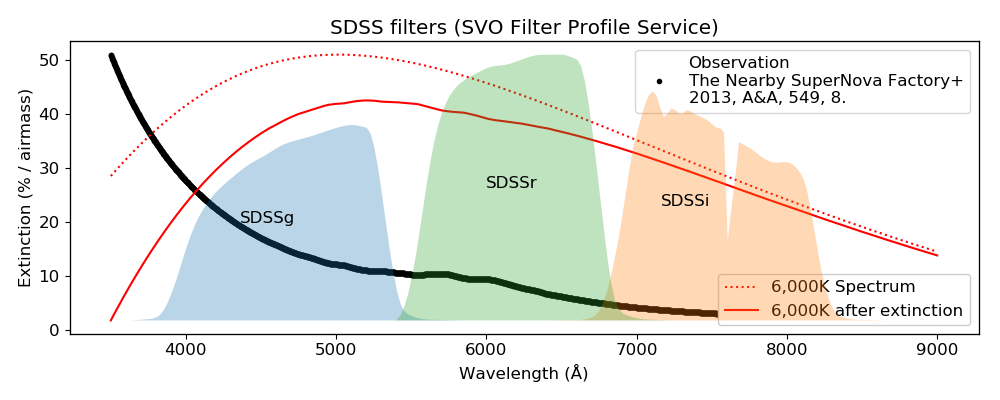
\includegraphics[width=0.9\linewidth]{figs/air-ext-bbrad}
\caption{A black body radiation spectrum ($ T = \SI{6000}{K} $) before and after the extinction at SDSS bands. Note that the y-axis is changed to \% per airmass (cf. \cref{fig:air-ext-and-filter}) by $ 10^{-0.4 \Delta m} $.}
\label{fig:air-ext-bbrad}
\end{figure}

As can be seen, \emph{the extinction is stronger for higher temperature (lower color index)}, so likely $ k_f'' < 0 $. However, the difference of extinction between the objects gets smaller as we look at longer wavelength. Thus, $ k_f'' \sim 0 $ except for B or u filters.

These facts can also be understood qualitatively. The higher the temperature the spectrum will have more fraction of energe at shorter wavelength. Considering that the atmospheric extinction is stronger at shorter wavelength (see black markers in \cref{fig:air-ext-bbrad}), high termperature object will get more ``penalty'' when it comes into the atmosphere. That is why high temperature object is more strongly extincted, i.e., $ k_f'' $ is negative. At the same time, since the amount of extinction drops significantly at wavelengths of r and i bands, and making $ k_f'' $ itself very small. 

SmithJA+ (2002, AJ, 123, 2121) determined the coefficients for SDSS filters at 1.0 m Ritchey--Chr\'{e}tien telescope at the USNO Flagstaff Station, from the observations in 1998--2000 in \cref{tab: SDSS ext}. The $ k_f' $ value fluctuates much for each night (see Fig 6 of the original publication), so I just took representative values from visual inspection. The $ k_f'' $ values were obtained by two independent pipelines, \texttt{superExcal} (method 1) and \texttt{solve\_network} (method 2). Both are quite consistent except for the u filter. The color $ C $ used for each filter is the nearby filter color: $ \mathrm{u}'-\mathrm{g}' $ for $ \mathrm{u}' $, $ \mathrm{g}'-\mathrm{r}' $ for $ \mathrm{g}' $, etc, and $ \mathrm{i}' - \mathrm{z}' $ for both $ \mathrm{i}' $ and $ \mathrm{z}' $. The atmospheric extinction coefficients $ (k_f',\, k_f'') $ all change as a function of time. We just hope they are reasonably constant during our observation of our targets and standard stars. From experience, we know $ k_f'' $ is always very small for filters longer than u or B-band, but is not necessarily ignorable because $ k_f'' XC $ might be larger than the accuracy you want to obtain. 


\begin{table}[ht!]
\caption{The extinction coefficients of SDSS from SmithJA+ (2002, AJ, 123, 2121).}
\label{tab: SDSS ext}
\centering
  \begin{tabular}{c||lllll}
  Parameter  & u$ ' $ & g$ ' $ & r$ ' $ & i$ ' $ & z$ ' $ \\
  \hline
  $ k_f' $ & $ > +0.5 $ & $ +0.20 \pm 0.05 $ & $ +0.10 \pm 0.05 $ & $ +0.05 \pm 0.05 $ & $ +0.05 \pm 0.05 $\\
  $ k_f'' $ method 1 
    & $ -0.021 \pm 0.003 $
    & $ -0.016 \pm 0.003 $ 
    & $ -0.004 \pm 0.003 $
    & $ +0.006 \pm 0.003 $ 
    & $ +0.003 \pm 0.003 $ \\
  $ k_f'' $ method 2
    & $ -0.032 $ 
    & $ -0.015 $
    &  $ 0.000 $
    & $ +0.005 $
    & $ +0.006 $
  \end{tabular}
\end{table}


%Atmosphere diminishes the flux of the object. For an optical depth of $ \tau $, an object with initial flux $ I_0 $ will be observed as $ I = I_0 e^{-\tau} $ and its magnitude will be increased (because flux is decreased) by $ \Delta m = -2.5 \lg (I / I_0) = \frac{2.5}{\lg e} \tau = 1.086 \tau $. But $ \tau = \int n \sigma dl $ for the number density of particles $ n $, the extinction cross-section $ \sigma $, and traveling distance $ l $. The total traveling distance, $ L $, is $ L_0 / \cos z = L_0 X $ where $ X $ is the airmass. Thus, a simple approximation that $ \tau \propto L $ will result in $ \Delta m \propto X $. 

%The real story is more complicated: This extinction is of course wavelength-dependent (\cref{fig:air-ext-and-filter}). The black markers show the extinction magnitude per airmass. At zenith, $ X = 1 $ by definition, so this means that $ \Delta m \sim \m{0.2} $ at $ \lambda = \SI{4000}{\AA} $ but is $ \Delta m \ll \m{0.1} $ for $ \lambda = \SI{8000}{\AA} $. Therefore, the extinction is not simply proportional to $ X $, but the proportionality is a function of wavelength.

%\begin{thm}[Atmospheric Extinction: 1st Order]
%The extinction due to the atmosphere has the following 1st order term:
%\begin{equation*}
%  \Delta m(\lambda) = k'(\lambda) X ~,
%\end{equation*}
%where $ k'(\lambda) $ is the first-order extinction coefficient and is a function of wavelength $ \lambda $. In photometry, we are dealing with filters rather than each single wavelength, so normally we denote 
%\begin{equation}\label{eq: air-ext 1st ord}
%  \Delta m_f = k_f' X ~.
%\end{equation}
%\end{thm}
 

%Consider a black body spectrum is underwent this atmospheric extinction: \cref{fig:air-ext-bbrad}. The extinction is of course a function of wavelength. 

%In photometry, we are interested in the total number of photons \textit{after} multiplied with the filter profile: $ \int_{\lambda_1}^{\lambda_2} S(\lambda) f(\lambda) d\lambda $ where $ S(\lambda) $ is the spectrum and $ f(\lambda) $ is the filter profile. Thus, the magnitude change before and after the atmospheric extinction is, if the extinction is $ E(\lambda) $,
%\begin{equation}
%  \Delta m = 
%    -2.5 \lg \qty (\frac{\int_{\lambda_1}^{\lambda_2} E(\lambda) S(\lambda) f (\lambda) d\lambda}{\int_{\lambda_1}^{\lambda_2} S(\lambda) f(\lambda) d\lambda} )
%\end{equation} 
%Because it contains a ratio of the integration, it is not simple to calculate $ \Delta m $. From target to target, what changes is, except for the airmass (Note that $ E(\lambda) = e^{-\tau} \propto \sim e^X $), the $ S(\lambda) $. Thus, $ \Delta m = \Delta m (X, S) $. For a black body, this is a function of the temperature, and the temperature has (roughly) one-to-one counterpart of the color index. Thus, if the spectral shape is assumed as black body, we can write $ \Delta m = \Delta m (X, C) $ where $ C $ is the true color index. Even if it is not a black body, it is sufficient if the spectral shape and color index have \textit{nearly} one-to-one relationship. The extinction due to the spectral shape should also be proportional to the airmass to the first order approximation. Thus, as an approximation, we add a term proportion to $ CX $ to  \cref{eq: air-ext 1st ord}:

%\begin{thm}[Atmospheric Extinction: 2nd Order]
%The extinction due to the atmosphere is:
%\begin{equation}
%  \Delta m(\lambda) = k'(\lambda) X + k''(\lambda) C X ~,
%\end{equation}
%where $ k''(\lambda) $ is the second order atmospheric extinction coefficient.
%In photometry, we are dealing with filters rather than each single wavelength, so normally we denote 
%\begin{equation}\label{eq: air-ext 2nd ord}
%  \Delta m_f = k_f' X + k_f'' C X ~.
%\end{equation}
%\end{thm}


\begin{ex}[Ignoring the Second Order Extinction Term]
Consider an observation at $ X = 2 $ of $ C = 0.2 $ star. If you ignore the second order extinction term, you are making $ k_f'' XC = 0.4 k_f'' $ of uncertainty. According to \cref{tab: SDSS ext}, this is most likely smaller than 0.01 magnitude. 

The Sun has $ C = \mathrm{g' - r'} \sim 0.5 $, and then the error for Sun-like star becomes $ 1.0 k_f'' $: It is $ < \m{0.01} $ for r, i, and z bands. It is about $ 0.02\mathrm{-}0.03 $ mag for $ \mathrm{u}' $.

The red M0 stars have $ C = \mathrm{g' - r'} \lesssim 1.5 $ and the error is now up to $ 3.0 k_f'' $. The accuracy of $ \m{0.01} $ can be achieved in riz bands, but risky.
\end{ex}

The calculation above is only for SDSS observatory at altitude of 2.3 km. But fortunately, BuchheimB (2005, SASS, 24, 111) found that the $ k_f'' \lesssim 0.005 $ for V band even at many low-altitude observatories (including Bochum observatory at altitude 200 m, Vainu Bappu Observatory at altitude 700 m), so likely we expect the correction from the second-order extinction term is small enough.


\subsection{Transformation Coefficient}
The sensitivity of the optics, such as filter, lens, mirror, and/or CCD cover glass, is also a function of $ \lambda $. The argument is identical to atmospheric extinction, but there is no $ X $ (similar parameter will be something like the optical depth of materials blocking CCD pixel, but that should be a device-dependent constant). Then the same logic leads us to the conclusion that there should be a color term which tunes the final output of the CCD count, and that is the $ \tilde{k}_f c $ (``transformation'') term. Here, $ c $ is the color index of the object after all the atmospheric extinction, and the true color before it enters telescopic optics. Once we assume there exists a function $ f_c $ such that $ f_c(C) = c $ is a one-to-one function and $ f_c(C) \approx \tilde{c}_5 + \tilde{c}_6 C $ for constants $ \tilde{c}_5 $ and $ \tilde{c}_6 $, the transformation term becomes $ k_f C + \tilde{c}_{7f} $ for the filter-dependent constant $ \tilde{c}_{7f} $. This constant is finally absorbed in to another filter-dependent constant, called the zero point, $ z_f $. Therefore we reach \cref{eq: std}.

The transformation coefficient, which I denoted $ k_f $, is fortunately nearly constant for the given device. Warner argues that it is enough to update $ k_f $ (Warner uses notation of $ T_f $) value only about 2--4 times a year, unless you physically changed the device elements (e.g., filter, CCD, lens, etc). Moreover, from experience, we know that this is nearly zero: $ |k_f| \lesssim 0.1 $. Many cases $ |k_f| \lesssim 0.01 $. Since the range of color indices are $ \mathrm{max}(\Delta C) \lesssim \m{1} $, we have $ |k_f C| \lesssim 0.1 $, and in many cases, $ |k_f C| \lesssim 0.01 $.


\subsection{A Note on Linearity} \label{ss: linearity note}
As we noted at the beginning part of this chapter, CCD is highly linear. That means, $ N = g N_e = \alpha N_\gamma $ where $ N $ is the pixel count (after \emph{bias} and \emph{dark} subtraction), $ N_e $ is the total number of photo-electrons, $ g $ is the electronic gain of the CCD (a constant; unit of counts per electrons), and $ N_\gamma $ is the photon incident to the CCD from the true photon number $ N_\mathrm{\gamma 0} $. No higher-order terms, no other constants. The $ \alpha $ value may differ from pixel to pixel due to the inhomogeneity of optics or CCD pixels, but they are homogeneized by the so-called \emph{flat fielding}, so here I can safely say it is strictly constant over all the pixels. 

Any kind of extinction (atmosphere or optics in front of the CCD) is multiplicative only to the linear term, i.e., $ N_\gamma = N_{\gamma 0} \times \mathrm{something_1} $ (e.g., $ e^{-\tau} $). There is neither higher-order terms like $ N_{\gamma 0}^2 $ nor addition of constant. Therefore, $ N = \mathrm{something_2} \times N_\mathrm{\gamma 0} $ and the instrumental magnitude
\begin{equation}
  m_f 
    := -2.5 \lg N 
    = \mathrm{something_3} - 2.5 \lg N_{\gamma 0}
    \equiv \mathrm{something_3} + M_f ~.
\end{equation} 
Thus, thanks to the linearity of CCD, we have \textbf{no additional coefficient \emph{multiplied}} in front of $ m_f $ or $ M_f $. If, for example, $ N $ were $ \alpha N_\gamma + \alpha' $, or there were other terms in the extinction (proportional to $ N^2 $ or a constant radiation from the optics), this simple relation wouldn't hold.

%In reality, the broad-band photometry (the  has some tricky problem. For a simple illustration, assume (1) we don't have atmosphere, (2) have a flat throughput: $ f(\lambda) = 1 $ for $ \lambda = [\lambda_1, \lambda_2] $ and zero otherwise, (3) CCD and optics has no wavelength-dependency in its sensitivity. We observed two stellar black-body spectra of temperatures $ T_a $ and $ T_b $ ($ T_a < T_b $). Because of different radii of or distance to the stars, consider they are shooting identical number of photons per time to Earth, i.e., $ \int_{\lambda_1}^{\lambda_2} S(\lambda) / (hc / \lambda) d\lambda $ is the same for two stars. The CCD will produce the same number of photo-electrons when it is hit by, e.g., 100 photons of $ \lambda_1 $ or 100 photons of $ \lambda_2 $. Thus, the two stars will appear to have identical brightness.

To emphasize, \emph{you should not worry about whether to \emph{multiply} something in front of $ M_f $ or $ m_f $ to satisfy \cref{eq: std}}. Their coefficients \emph{must be unity}. From our experiences, most observational experts and electrical engineers would say that you should only care about this if you are sure that some parts of the optics have serious problems (e.g., your CCD underwent serious problem and shows non-linearity). 

\subsection{A Note on Zero Point} \label{ss: zeropt}
The zero point $ z_{f} $ is a constant to convert the instrumental magnitude (which is nothing but a $ -2.5 $ multiplied by $ \lg (\mathrm{count}) $) to a realistic standard magnitude system astronomers have been using. In intensity sence, this ``addition of a constant'' in magnitude represents a ``multiplication of a constant'' to the instrumental count to measure the intensity. 

% !!!!!!!!!!!!!!!!!!!!!!!!!!!!!!!!!!!!!!!!!!!!!!!!!!!!!!!!!!!!!!!!!!!!!!!!!!!!!!!!
% !!!!!!!!!!!!!!!!!!!!!!!!!!!!!!!!!!!!!!!!!!!!!!!!!!!!!!!!!!!!!!!!!!!!!!!!!!!!!!!!
% !!!!!!!!!!!!!!!!!!!!!!!!!!!!!!!!!!!!!!!!!!!!!!!!!!!!!!!!!!!!!!!!!!!!!!!!!!!!!!!!
% !!!!!!!!!!!!!!!!!!!!!!!!!!!!!!!!!!!!!!!!!!!!!!!!!!!!!!!!!!!!!!!!!!!!!!!!!!!!!!!!
% add photon/sec for 0-mag star from Ishiguro's notebook and do realistic calculation
% !!!!!!!!!!!!!!!!!!!!!!!!!!!!!!!!!!!!!!!!!!!!!!!!!!!!!!!!!!!!!!!!!!!!!!!!!!!!!!!!
% !!!!!!!!!!!!!!!!!!!!!!!!!!!!!!!!!!!!!!!!!!!!!!!!!!!!!!!!!!!!!!!!!!!!!!!!!!!!!!!!
% !!!!!!!!!!!!!!!!!!!!!!!!!!!!!!!!!!!!!!!!!!!!!!!!!!!!!!!!!!!!!!!!!!!!!!!!!!!!!!!!
% !!!!!!!!!!!!!!!!!!!!!!!!!!!!!!!!!!!!!!!!!!!!!!!!!!!!!!!!!!!!!!!!!!!!!!!!!!!!!!!!

What is a typical value of zero point? From telescopes with diameter $ \gtrsim \SI{1}{m} $ in Seoul, let's say we are observing objects of around $ \m{15} $ with 100 seconds exposure. Say the sky-subtracted peak value of our target is\footnote{Because CCDs are usually operated in 16-bit unsigned integer mode which represents $ 0 $ to $ 65,535 $, and non-linearity appears around $ 40,000 $, the sky subtracted peak pixel value of an intermediate-brightness object in the FOV is order of $ \sim 10^4 $ after sky subtraction} $ \sim 10^4 $ and the integral of the profile gives intensity of $ \sim 10^{5} $, and the intensity per unit time is $ 10^3 $ (divided by exposure time). The instrumental magnitude is $ m \sim -2.5 \lg 10^3 = -7.5 $. This means $ z_f \sim 22.5 $. If we do realistic calculation, $ z_f $ is mostly within a range of 20 to 25. This is why, in IRAF, the default initial guess of $ z_f $ is 25 mag.

Zero point must be a constant unless the device is affected by external disturbance in our simple model dealt in this chapter. In reality it is true that this zero point fluctuate at each exposure, and that is because of the imperfect readout process of CCD electronics. $ \Delta z_\mathrm{V} \approx 0 $ is assumed in this chapter. Although you may be unconfortable, but this is what is assumed even in professional space telescope data reduction processes, if this fact makes you more comfortable.

\section{Standardization Applied to Photometry}
Now that we justified the usage of \cref{eq: std}, let's find the cases of application. The simplest case is the \textit{differential photometry}. 

If there are many celestial objects (of course including your target) in the field of view with known standard magnitudes, we can use them as standard stars. Although there can be variable stars and galaxies\footnote{Galaxies can have spectra significantly different from those of black bodies. Therefore, the coefficients $ k_f $ and $ k_f'' $, which are approximations of spectral shape (i.e., not $ k_f' $), should be different from those derived from standard \textit{stars}, which are black bodies to the first order. But mostly this effect is not serious because, as we discussed before, both $ k_f C $ and $ k_f'' X C $ terms are anyway very small. For this reason, people use $ k_f $ and $ k_f'' $ derived from standard stars for their target galaxies (or any non-black body like spectra). If you really worry about this, you must conduct spectroscopic observation, not broad-band photometry.}, if most of the objects with known magnitudes are non-variable stars, those \textit{outliers} will be smoothed out. Thus, we just assume all the celestial objects in the field of view with known standard magnitudes as ``standard stars''. 

This technique is very widely used in variable star and asteroidal light curve observations. This is widely used than absolute photometry, because it is annoying and difficult to observe standard stars at different airmasses while observing your target, which requires telescope time and human labor. In asteroidal science, even single-filter differential photometry is frequently used. 

\subsection{Differential Photometry: Single-Filter}

Consider there are many stars in the FOV with known (catalogued) magnitudes at multiple filters, so that the true apparent magnitude $ M_f $ and color $ C $ are known. Say, from the photometry, we could determine the instrumental magnitude of stars $ m_f $. Rearranging \cref{eq: std}:
\begin{equation} \label{eq: zeropt}
  M_f - m_f = (z_f - k_f' X) + (k_f - k_f'' X) C \equiv a_f (X) + b_f (X) C
\end{equation}
The first term in the RHS, $ a_f (X) $, is a constant for all the stars in the same FITS frame, as they will have nearly identical airmass\footnote{If you observed near the horizon, $ \Delta X $ across the FOV may not be negligible. For accurate photometry, this should also be taken into account.} $ X $ and the identical zero point $ z_f $. $ M_f - m_f = a_f(X) $ for $ C = 0 $, i.e., a perfectly flat spectrum. The second term is color-dependent, but as we discussed before, it is likely to be very small. Sometimes people just call this value (LHS) as ``zero point'', although I will stick to use this term for $ z_f $ for clarity. 

\begin{ex}[How small is the second term?]
  Consider observatinos made in wavelength ranges around V or gri bands. From \cref{tab: SDSS ext}, $ |k_f''| \sim 0.000 \mathrm{-} 0.020 $ and we expect that $ k_f \lesssim 0.02 $ for most optics. Since $ k_f'' $ is mostly negative, $ k_f - k_f'' X $ is likely be positive, but not always (see \cref{tab: SDSS ext}). Also we have $ 1 < X \lesssim 2 $ in most cases. Then if you play with many combinations of numbers, $ b_f(X) C = (k_f - k_f'' X) C \lesssim 0.05 C $ and most likely much smaller than that. Note that the color index is mostly $ -1 \lesssim C \lesssim +1 $.
\end{ex}

What we do now is to draw several test plots as in \cref{fig:zeropt}. It is better if the color of the stars span wider than about 0.5 ($ \mathrm{max}(C) - \mathrm{min} (C) \gtrsim 0.5 $). On the left side of the figure, I plotted $ M_f $ VS $ m_f $ for $ f = \mathrm{R} $ (Johnson--Cousins $ \mathrm{R_C} $ filter). The fitted slope is $ \sim 1.015 $, which is near the unity as we expect from linearity. Sometimes it becomes as high as 1.05 throughout the night. Below is a residual plot. Normally, since the uncertainty in the magnitude measurement increases for larger magnitude (fainter star), the scatter of the residual must increase at large magnitude. The right panel of the figure shows the residual as a function of catalogued stars. The color-dependent slope is 0.02, and it was $ \lesssim 0.05 $ throughout the night; this is small indeed as we expected above. As we do not know our target's color, assuming the color uncertainty of $ \pm 0.5 $ will give around $ \pm 0.03 $ \textbf{\emph{systematic offset to the magnitude}} of our target. Note that this is a systematic parallel shift in magnitude, not a random error. Therefore, the \emph{shape} of the light curve will not be affected by this, althought the magnitude \emph{value} may have been affected by a constant.

\begin{figure}[ht!]
\centering
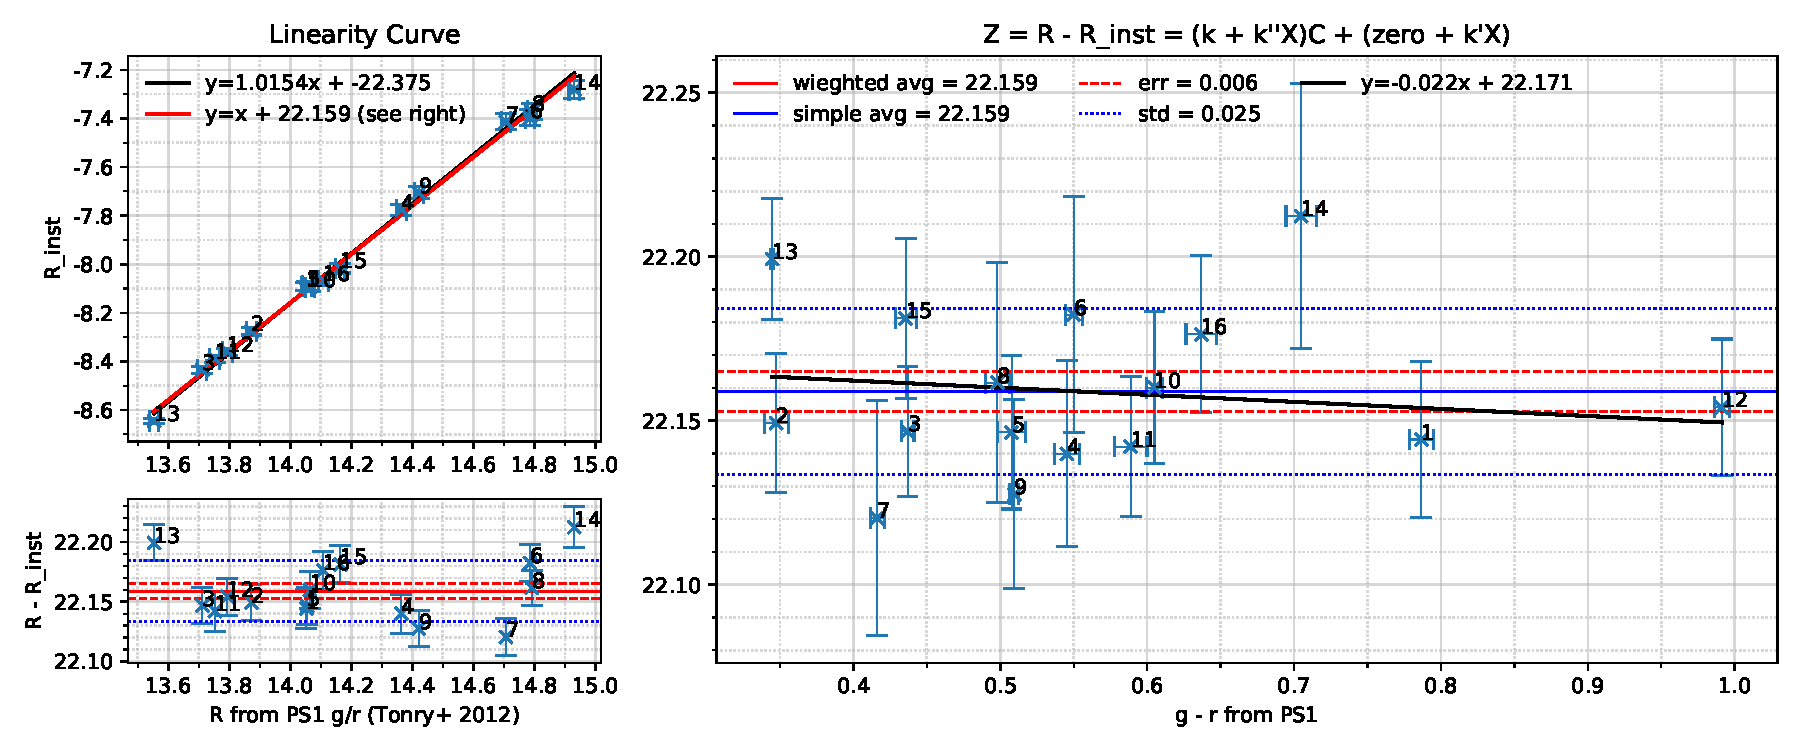
\includegraphics[width=\linewidth]{figs/SNUO_STX16803-2005UD-1-1-20181012-190829_zeropoint.pdf}
\caption{A typical linearity curve with residual (left) and color-zero plot (right) on 2018-10-12 (UT 19:08:29) observation at SNUO 1-m telescope for the field stars near an asteroid (155140) 2005 UD. I used PS1 DR1 catalog, within 13.5 to 15 mag, removed any object with flag of quasar, variable, galaxy, etc, and dropped any pairs of stars if there's any nearby object in PS1 DR1 catalog.}
\label{fig:zeropt}
\end{figure}

A summary of the three plots:
\begin{table}[ht!]
\caption{Differential Photometry Diagnostic Plots}
\label{tab: 1-filter diff phot}
\centering
  \begin{tabular}{c|cc|c|l}
  Name & $ x $-axis & $ y $-axis & Appearance & Comments \\
  \hline
  Linearity & $ M_f $ & $ m_f $       & straight line & 
  $ |\mathrm{slope} - 1| \gtrsim 0.01 $ means you need to \\
  Curve & & & slope of unity & check your photometry and/or device linerity \\
  \hline
  Linearity & $ M_f $ & $ M_f - m_f $ & constant value & 
  Scatter is larger for large $ M_f $ objects \\
  Residual & & & regardless of $ M_f $ & ($ \because $ faint object's mag is less accurate) \\
  \hline
  Color & $ C $  & $ M_f - m_f $ & $ \sim $ constant & 
  If you can see a clear trend, \\
  Dependency & & & regardless of $ M_f $ & the color-terms in \cref{eq: zeropt} not negligible.\\
\end{tabular}
\end{table}

If graphs do not look as expected, that means (1) many field objects are variable or highly non-blackbody-like galaxies so that they are not suitable as ``standard stars'' and the basic assumptions of \cref{eq: std} break down, (2) the airmass is too high that the 2nd order approximations do not hold, (3) catalog $ M_f $ suffer from unknown uncertainties or systematic errors so the catalog value is not reliable, (4) $ m_f $ was measured incorrectly, (5) many other possibilities. Check these before going further, because your final results may be affected.


Consider you determined the $ (a_f, b_f) $ for all the FITS files you obtained through a night, where each FITS file has different airmass. Then, if you 
\begin{itemize}
\item plot $ a_f $ as $ X $, the intercept and slope are $ z_f $ and $ -k_f' $,
\item plot $ b_f $ as $ X $, the intercept and slope are $ k_f $ and $ -k_f'' $.
\end{itemize}

Note, however, the following assumptions should be met: 
\begin{enumerate}
\item Atmospheric conditions (extinction coefficients $ k' $ and $ k'' $), remain constant over the night 
\item Zero point $ z_f $ remain constant over the night 
\item The approximations used for \cref{eq: std} (2nd-order approximation) must hold
\end{enumerate}

Because not all these are met in Seoul sky, the plots you made will not look like to have a linear trend. It can be largely scattered so that a linear fit does not seem to make sense, clear non-linear trend appears (mostly due to the third assumption breaks down at large airmass), etc.

Therefore, as a simple yet reasonable approximation, I assumed $ M_f - m_f $ for all the objects in a single FITS file should be a constant, and found this value. Then added it to the instrumental magnitude $ m_f $ of the target of interest.


\subsection{Differential Photometry: Multi-Filter}
When we have more than one filter observation, we can even eliminate the systematic offset due to the color uncertainty of the object. Just write the equation for two filters, $ x $ and $ y $
\begin{equation}
\begin{cases}
  M_x - m_x &= (z_x - k_x' X_x) + (k_x - k_x''X_x) C_{xy} = a_x(X_x) + b_x(X_x) C_{xy} \\
  M_y - m_y &= (z_y - k_y' X_y) + (k_y - k_y''X_y) C_{xy} = a_y(X_y) + b_y(X_y) C_{xy} 
\end{cases}
\end{equation}
Note here that, for field stars with known standard magnitudes, $ M_x $, $ M_y $, and thus $ C_{xy} = M_x - M_y $ should all be known. The $ m_x $ and $ m_y $ are known from a photometry to the image. Although $ z $ values are assumed to be constant throughout the night for the same detector, I explicitly put $ z_x $ and $ z_y $ for generality. Following the logic of single-filter case, if we plot $ M_x - m_x $ as ordinate and $ C_{xy} $ as abscissa for $ N $ field stars, the $ y $-intercept is $ a_x $ and the slope is $ b_x $. Same goes for the $ y $ filter. So  $ (a_x, b_x) $ and $ (a_y, b_y) $ are determined with the uncertainties.

Then for the target of interest, which $ M_x $ and $ M_y $ are unknown,
\begin{equation}
\begin{cases}
  M_x^\mathrm{target} - m_x^\mathrm{target} &= a_x(X_x) + b_x(X_x) C_{xy}^\mathrm{target} \\
  M_y^\mathrm{target} - m_y^\mathrm{target} &= a_y(X_y) + b_y(X_y) C_{xy}^\mathrm{target}
\end{cases}
\end{equation}
or since $ C_{xy}^\mathrm{target} = M_x^\mathrm{target} - M_y^\mathrm{target} $, (dropping $ X_x $ and $ X_y $ for brevity)
\begin{equation}
  C_{xy}^\mathrm{target} = \frac{(m_x^\mathrm{target} - m_y^\mathrm{target}) + (a_x - a_y)}{1 - (b_x - b_y)} ~.
\end{equation}
Putting this back to the original equation,
\begin{equation}\label{eq: 2-filter diff phot sol}
\begin{cases}
  M_x^\mathrm{target}
    = m_x + a_x + b_x \frac{(m_x^\mathrm{target} - m_y^\mathrm{target}) + (a_x - a_y)}{1 - (b_x - b_y)} \\
  M_y^\mathrm{target}
    = m_y + a_y + b_y \frac{(m_x^\mathrm{target} - m_y^\mathrm{target}) + (a_x - a_y)}{1 - (b_x - b_y)}
\end{cases}
\end{equation}
Now we have the standard magnitude of the target in both $ x $ and $ y $ filters. Since we have taken the color of the target into account, \textbf{\emph{there is no systematic offset}} as in single-filter case.

What if we have more than 2 filters, say $ x $, $ y $, and $ z $? Solve for $ x $ and $ y $ as above by using $ (a_x, b_x) $. Then solve for $ y $ and $ z $, but this time using color as $ C_{yz} $, not $ C_{xy} $, using $ (a_y', b_y') $. Theoretically $ a_y = a_y' $, because there is no color term. However, $ b_x \neq b_x' $, because $ k_y'' $ is defined for $ C_{xy} $ for the first case, but it is defined for $ C_{yz} $ for the second case. In reality, because what we get is only the best-fit values with uncertainties, $ a_x $ and $ a_x' $ can also be different (likely within certain amount of error-bar).




\section{Photometry Using Standard Stars}
When we need accurate absolute photometry, photometric standard star observation is essential. Unlike ``field stars with known magnitude,'' standard stars are confirmed as non-variable stars with very accurate magnitudes. By observing them, we determine the coefficients ($ k_f $, $ k_f' $, and $ k_f'' $) and zero point ($ z_f $), mostly for at least two filters, and get the magnitude of our target of interest with high accuracy. Hence, I will only talk about multi-filter observation of standard stars.

A different thing for standard star frames is that there is only one star with known magnitude in the FOV, and there will be only one point in the right panel of \cref{fig:zeropt}. Therefore, we select at least two standard stars with different colors, sometimes called a \textbf{\emph{blue--red pair}}. Observe one standard star at an airmass. When the other standard star reaches similar airmass, observe it, so that you have at least two stars at the same airmass. Then you have two points in the right panel of \cref{fig:zeropt} at the given airmass. Repeat this for many airmasses, so that you obtain the $ a_f $ and $ b_f $ for many airmasses for each filter. Following the logic of multi-filter case, you can determine all the coefficients.

If you are not interested in zero point and the transformation coefficient $ k_f $, you can follow this calculation: Consider a standard star with ID $= i $ is observed for $ N_i $ times, and denote each observation as $ j $ $ (j = 1, \cdots, N_i) $, and write the parameters of \cref{eq: std} as $ M_{f, i} $, $ C_{i} $ ($ M $ and $ C $ are fixed values for a standard star, so no $ j $ is needed), $ m_{f, i}^{(j)} $, $ X_{f, i}^{(j)} $, etc. We here assume the zero point, $ z_f $, and the coefficients $ k_f $, $ k_f' $, and $ k_f'' $ are almost constant over the night\footnote{Even SDSS standard stars were also observed and analyzed under this assumption. See SmithJA (2002, AJ, 123, 2121)}. Then
\begin{equation}
\begin{cases}
  M_{f, i} - m_{f, i}^{(1)}
    &= z_f + k_f' X_{f, i}^{(1)} + k_f'' X_{f, i}^{(1)} C_{i} + k_f C_{i} ~, \\
  M_{f, i} - m_{f, i}^{(2)}
    &= z_f + k_f' X_{f, i}^{(2)} + k_f'' X_{f, i}^{(2)} C_{i} + k_f C_{i} ~, \\
  \qquad\vdots & \qquad\vdots \\
  M_{f, i} - m_{f, i}^{(N_i)}
    &= z_f + k_f' X_{f, i}^{(N_i)} + k_f'' X_{f, i}^{(N_i)} C_{i} + k_f C_{i}   ~.
\end{cases}
\end{equation}
For the first two observations of the same standard star (ID $= i $) at filter $ f $, subtracting two,
\begin{equation}
  \Delta m_{f, i}^{(1, 2)} 
    = (k_f' + k_f'' C_i) \Delta X_{f, i}^{(1, 2)} 
  \quad\rightarrow\quad
  \qty( \frac{\Delta m }{\Delta X} )_{f, i}^{(1, 2)}
    = k_f' + k_f'' C_i ~.
\end{equation}
Of course $ \Delta m_{f, i}^{(1, 2)}  = m_{f, i}^{(1)} - m_{f, i}^{(2)} $ and $ \Delta X_{f, i}^{(1, 2)}  = X_{f, i}^{(1)} - X_{f, i}^{(2)} $. 

Therefore, if we plot $ \qty ( \frac{\Delta m }{\Delta X} )_{f, i} $ as a function of color $ C_i $ of the standard stars with different color indices (colors of them are all known), the linear fit will give intercept of $ k_f' $ and slope of $ k_f'' $. For star $ i $, we have $ N_i $ observations, so we have $ \binom{N_i}{2} = N_i (N_i - 1) / 2 $ points at the single $ C_i $ value. If we have $ N $ standard stars of wide color range, we can have $ N \sum_i \binom{N_i}{2} $ points to fit the linear line. For a simple blue--red pair, $ N = 2 $, so you have two $ x $-axis values (color index), but many points at each $ x $-axis value.

